%\begin{Shaded}
%\begin{Highlighting}[]
%\KeywordTok{library}\NormalTok{(AnnotationHub)}
%\NormalTok{ah \textless{}{-}}\StringTok{ }\KeywordTok{AnnotationHub}\NormalTok{()}
%\NormalTok{tag =}\StringTok{ }\KeywordTok{names}\NormalTok{(}\KeywordTok{query}\NormalTok{(ah, }\KeywordTok{c}\NormalTok{(}\StringTok{"Ensembl"}\NormalTok{,}\StringTok{"110"}\NormalTok{, }\StringTok{"Homo sapiens"}\NormalTok{)))}
%\NormalTok{ens110 \textless{}{-}}\StringTok{ }\NormalTok{ah[[tag]]}
%\end{Highlighting}
%\end{Shaded}


\section{Section Heading}
\label{sec:1}
Use the template \emph{chapter.tex} together with the document class SVMono (monograph-type books) or SVMult (edited books) to style the various elements of your chapter content.

Instead of simply listing headings of different levels we recommend to let every heading be followed by at least a short passage of text.  Further on please use the \LaTeX\ automatism for all your cross-references and citations. And please note that the first line of text that follows a heading is not indented, whereas the first lines of all subsequent paragraphs are.

\section{Section Heading}
\label{sec:2}
% Always give a unique label
% and use \ref{<label>} for cross-references
% and \cite{<label>} for bibliographic references
% use \sectionmark{}
% to alter or adjust the section heading in the running head
Instead of simply listing headings of different levels we recommend to let every heading be followed by at least a short passage of text.  Further on please use the \LaTeX\ automatism for all your cross-references and citations.

Please note that the first line of text that follows a heading is not indented, whereas the first lines of all subsequent paragraphs are.

Use the standard \verb|equation| environment to typeset your equations, e.g.
%
\begin{equation}
a \times b = c\;,
\end{equation}
%
however, for multiline equations we recommend to use the \verb|eqnarray| environment\footnote{In physics texts please activate the class option \texttt{vecphys} to depict your vectors in \textbf{\itshape boldface-italic} type - as is customary for a wide range of physical subjects}.
\begin{eqnarray}
\left|\nabla U_{\alpha}^{\mu}(y)\right| &\le&\frac1{d-\alpha}\int
\left|\nabla\frac1{|\xi-y|^{d-\alpha}}\right|\,d\mu(\xi) =
\int \frac1{|\xi-y|^{d-\alpha+1}} \,d\mu(\xi)  \\
&=&(d-\alpha+1) \int\limits_{d(y)}^\infty
\frac{\mu(B(y,r))}{r^{d-\alpha+2}}\,dr \le (d-\alpha+1)
\int\limits_{d(y)}^\infty \frac{r^{d-\alpha}}{r^{d-\alpha+2}}\,dr
\label{eq:01}
\end{eqnarray}

\subsection{Subsection Heading}
\label{subsec:2}
Instead of simply listing headings of different levels we recommend to let every heading be followed by at least a short passage of text.  Further on please use the \LaTeX\ automatism for all your cross-references\index{cross-references} and citations\index{citations} as has already been described in Sect.~\ref{sec:2}.

\begin{quotation}
Please do not use quotation marks when quoting texts! Simply use the \verb|quotation| environment -- it will automatically be rendered in line with the preferred layout.
\end{quotation}


\subsubsection{Subsubsection Heading}
Instead of simply listing headings of different levels we recommend to let every heading be followed by at least a short passage of text.  Further on please use the \LaTeX\ automatism for all your cross-references and citations as has already been described in Sect.~\ref{subsec:2}, see also Fig.~\ref{fig:1}\footnote{If you copy text passages, figures, or tables from other works, you must obtain \textit{permission} from the copyright holder (usually the original publisher). Please enclose the signed permission with the manuscript. The sources\index{permission to print} must be acknowledged either in the captions, as footnotes or in a separate section of the book.}

Please note that the first line of text that follows a heading is not indented, whereas the first lines of all subsequent paragraphs are.

% For figures use
%
\begin{figure}[b]
\sidecaption
% Use the relevant command for your figure-insertion program
% to insert the figure file.
% For example, with the graphicx style use
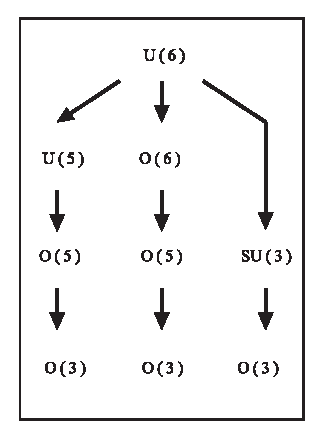
\includegraphics[scale=.65]{figure}
%
% If no graphics program available, insert a blank space i.e. use
%\picplace{5cm}{2cm} % Give the correct figure height and width in cm
%
\caption{If the width of the figure is less than 7.8 cm use the \texttt{sidecapion} command to flush the caption on the left side of the page. If the figure is positioned at the top of the page, align the sidecaption with the top of the figure -- to achieve this you simply need to use the optional argument \texttt{[t]} with the \texttt{sidecaption} command}
\label{fig:1}       % Give a unique label
\end{figure}


\paragraph{Paragraph Heading} %
Instead of simply listing headings of different levels we recommend to let every heading be followed by at least a short passage of text.  Further on please use the \LaTeX\ automatism for all your cross-references and citations as has already been described in Sect.~\ref{sec:2}.

Please note that the first line of text that follows a heading is not indented, whereas the first lines of all subsequent paragraphs are.

For typesetting numbered lists we recommend to use the \verb|enumerate| environment -- it will automatically rendered in line with the preferred layout.

\begin{enumerate}
\item{Livelihood and survival mobility are oftentimes coutcomes of uneven socioeconomic development.}
\begin{enumerate}
\item{Livelihood and survival mobility are oftentimes coutcomes of uneven socioeconomic development.}
\item{Livelihood and survival mobility are oftentimes coutcomes of uneven socioeconomic development.}
\end{enumerate}
\item{Livelihood and survival mobility are oftentimes coutcomes of uneven socioeconomic development.}
\end{enumerate}


\subparagraph{Subparagraph Heading} In order to avoid simply listing headings of different levels we recommend to let every heading be followed by at least a short passage of text. Use the \LaTeX\ automatism for all your cross-references and citations as has already been described in Sect.~\ref{sec:2}, see also Fig.~\ref{fig:2}.

For unnumbered list we recommend to use the \verb|itemize| environment -- it will automatically be rendered in line with the preferred layout.

\begin{itemize}
\item{Livelihood and survival mobility are oftentimes coutcomes of uneven socioeconomic development, cf. Table~\ref{tab:1}.}
\begin{itemize}
\item{Livelihood and survival mobility are oftentimes coutcomes of uneven socioeconomic development.}
\item{Livelihood and survival mobility are oftentimes coutcomes of uneven socioeconomic development.}
\end{itemize}
\item{Livelihood and survival mobility are oftentimes coutcomes of uneven socioeconomic development.}
\end{itemize}

\begin{figure}[t]
\sidecaption[t]
% Use the relevant command for your figure-insertion program
% to insert the figure file.
% For example, with the option graphics use
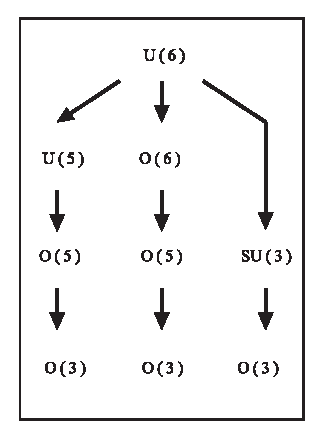
\includegraphics[scale=.65]{figure}
%
% If no graphics program available, insert a blank space i.e. use
%\picplace{5cm}{2cm} % Give the correct figure height and width in cm
%
%\caption{Please write your figure caption here}
\caption{If the width of the figure is less than 7.8 cm use the \texttt{sidecapion} command to flush the caption on the left side of the page. If the figure is positioned at the top of the page, align the sidecaption with the top of the figure -- to achieve this you simply need to use the optional argument \texttt{[t]} with the \texttt{sidecaption} command}
\label{fig:2}       % Give a unique label
\end{figure}

\runinhead{Run-in Heading Boldface Version} Use the \LaTeX\ automatism for all your cross-references and citations as has already been described in Sect.~\ref{sec:2}.

\subruninhead{Run-in Heading Boldface and Italic Version} Use the \LaTeX\ automatism for all your cross-refer\-ences and citations as has already been described in Sect.~\ref{sec:2}\index{paragraph}.

\subsubruninhead{Run-in Heading Displayed Version} Use the \LaTeX\ automatism for all your cross-refer\-ences and citations as has already been described in Sect.~\ref{sec:2}\index{paragraph}.
% Use the \index{} command to code your index words
%
% For tables use
%
\begin{table}[!t]
\caption{Please write your table caption here}
\label{tab:1}       % Give a unique label
%
% Follow this input for your own table layout
%
\begin{tabular}{p{2cm}p{2.4cm}p{2cm}p{4.9cm}}
\hline\noalign{\smallskip}
Classes & Subclass & Length & Action Mechanism  \\
\noalign{\smallskip}\svhline\noalign{\smallskip}
Translation & mRNA$^a$  & 22 (19--25) & Translation repression, mRNA cleavage\\
Translation & mRNA cleavage & 21 & mRNA cleavage\\
Translation & mRNA  & 21--22 & mRNA cleavage\\
Translation & mRNA  & 24--26 & Histone and DNA Modification\\
\noalign{\smallskip}\hline\noalign{\smallskip}
\end{tabular}
$^a$ Table foot note (with superscript)
\end{table}
%
\section{Section Heading}
\label{sec:3}
% Always give a unique label
% and use \ref{<label>} for cross-references
% and \cite{<label>} for bibliographic references
% use \sectionmark{}
% to alter or adjust the section heading in the running head
Instead of simply listing headings of different levels we recommend to let every heading be followed by at least a short passage of text.  Further on please use the \LaTeX\ automatism for all your cross-references and citations as has already been described in Sect.~\ref{sec:2}.

Please note that the first line of text that follows a heading is not indented, whereas the first lines of all subsequent paragraphs are.

If you want to list definitions or the like we recommend to use the enhanced \verb|description| environment -- it will automatically rendered in line with the preferred layout.

\begin{description}[Type 1]
\item[Type 1]{That addresses central themes pertainng to migration, health, and disease. In Sect.~\ref{sec:1}, Wilson discusses the role of human migration in infectious disease distributions and patterns.}
\item[Type 2]{That addresses central themes pertainng to migration, health, and disease. In Sect.~\ref{subsec:2}, Wilson discusses the role of human migration in infectious disease distributions and patterns.}
\end{description}

\subsection{Subsection Heading} %
In order to avoid simply listing headings of different levels we recommend to let every heading be followed by at least a short passage of text. Use the \LaTeX\ automatism for all your cross-references and citations citations as has already been described in Sect.~\ref{sec:2}.

Please note that the first line of text that follows a heading is not indented, whereas the first lines of all subsequent paragraphs are.

\begin{svgraybox}
If you want to emphasize complete paragraphs of texts we recommend to use the newly defined class option \verb|graybox| and the newly defined environment \verb|svgraybox|. This will produce a 15 percent screened box 'behind' your text.

If you want to emphasize complete paragraphs of texts we recommend to use the newly defined class option and environment \verb|svgraybox|. This will produce a 15 percent screened box 'behind' your text.
\end{svgraybox}


\subsubsection{Subsubsection Heading}
Instead of simply listing headings of different levels we recommend to let every heading be followed by at least a short passage of text.  Further on please use the \LaTeX\ automatism for all your cross-references and citations as has already been described in Sect.~\ref{sec:2}.

Please note that the first line of text that follows a heading is not indented, whereas the first lines of all subsequent paragraphs are.

\begin{theorem}
Theorem text goes here.
\end{theorem}
%
% or
%
\begin{definition}
Definition text goes here.
\end{definition}

\begin{proof}
%\smartqed
Proof text goes here.
%\qed
\end{proof}

\paragraph{Paragraph Heading} %
Instead of simply listing headings of different levels we recommend to let every heading be followed by at least a short passage of text.  Further on please use the \LaTeX\ automatism for all your cross-references and citations as has already been described in Sect.~\ref{sec:2}.

Note that the first line of text that follows a heading is not indented, whereas the first lines of all subsequent paragraphs are.
%
% For built-in environments use
%
\begin{theorem}
Theorem text goes here.
\end{theorem}
%
\begin{definition}
Definition text goes here.
\end{definition}
%
\begin{proof}
%\smartqed
Proof text goes here.
%\qed
\end{proof}
%
\begin{trailer}{Trailer Head}
If you want to emphasize complete paragraphs of texts in an \verb|Trailer Head| we recommend to
use  \begin{verbatim}\begin{trailer}{Trailer Head}
...
\end{trailer}\end{verbatim}
\end{trailer}
%
\begin{questype}{Questions}
If you want to emphasize complete paragraphs of texts in an \verb|Questions| we recommend to
use  \begin{verbatim}\begin{questype}{Questions}
...
\end{questype}\end{verbatim}
\end{questype}
\eject%
\begin{important}{Important}
If you want to emphasize complete paragraphs of texts in an \verb|Important| we recommend to
use  \begin{verbatim}\begin{important}{Important}
...
\end{important}\end{verbatim}
\end{important}
%
\begin{warning}{Attention}
If you want to emphasize complete paragraphs of texts in an \verb|Attention| we recommend to
use  \begin{verbatim}\begin{warning}{Attention}
...
\end{warning}\end{verbatim}
\end{warning}

\begin{programcode}{Program Code}
If you want to emphasize complete paragraphs of texts in an \verb|Program Code| we recommend to
use

\verb|\begin{programcode}{Program Code}|

\verb|\begin{verbatim}...\end{verbatim}|

\verb|\end{programcode}|

\end{programcode}
%
\begin{tips}{Tips}
If you want to emphasize complete paragraphs of texts in an \verb|Tips| we recommend to
use  \begin{verbatim}\begin{tips}{Tips}
...
\end{tips}\end{verbatim}
\end{tips}
\eject
%
\begin{overview}{Overview}
If you want to emphasize complete paragraphs of texts in an \verb|Overview| we recommend to
use  \begin{verbatim}\begin{overview}{Overview}
...
\end{overview}\end{verbatim}
\end{overview}
\begin{backgroundinformation}{Background Information}
If you want to emphasize complete paragraphs of texts in an \verb|Background|
\verb|Information| we recommend to
use

\verb|\begin{backgroundinformation}{Background Information}|

\verb|...|

\verb|\end{backgroundinformation}|
\end{backgroundinformation}
\begin{legaltext}{Legal Text}
If you want to emphasize complete paragraphs of texts in an \verb|Legal Text| we recommend to
use  \begin{verbatim}\begin{legaltext}{Legal Text}
...
\end{legaltext}\end{verbatim}
\end{legaltext}
%
\begin{acknowledgement}
If you want to include acknowledgments of assistance and the like at the end of an individual chapter please use the \verb|acknowledgement| environment -- it will automatically be rendered in line with the preferred layout.
\end{acknowledgement}
%
\ethics{Competing Interests}{Please declare any competing interests
in the context of your chapter. The following sentences can be regarded as examples.\newline
This study was funded by [X] [grant number X].\newline
 [Author A] has a received research grant from [Company W].\newline
 [Author B] has received a speaker honorarium from [Company X] and owns stock in [Company~Y].\newline 
 [Author C] is a member of [committee Z].\newline 
The authors have no conflicts of interest to declare that are relevant to the content of this chapter.}

\eject

\ethics{Ethics Approval}{If your chapter includes primary studies with humans please declare the adherence of ethical standards. Example text: This study was performed in line with the principles of the Declaration of Helsinki. Approval was granted by the Ethics Committee of University B (Date.../No. ...).\newline 
 In addition, for human participants, authors are required to include a statement that informed consent (to participate and/or to publish) was obtained from individual participants or parents/guardians if the participant is minor or incapable.\newline
If animals are studied, authors should make sure that the legal requirements or guidelines in the country and/or state or province for the care and use of animals have been followed or specify that no ethics approval was required.}

\section*{Appendix}
\addcontentsline{toc}{section}{Appendix}
%
%
When placed at the end of a chapter or contribution (as opposed to at the end of the book), the numbering of tables, figures, and equations in the appendix section continues on from that in the main text. Hence please \textit{do not} use the \verb|appendix| command when writing an appendix at the end of your chapter or contribution. If there is only one the appendix is designated ``Appendix'', or ``Appendix 1'', or ``Appendix 2'', etc. if there is more than one.

\cite{ref-Aevermann2018} is our latest.

\begin{equation}
a \times b = c
\end{equation}

\begin{thebibliography}{99.}%

\bibitem{ref-Aevermann2018}
Aevermann, Brian D., Mark Novotny, Trygve Bakken, Jeremy A. Miller, Alexander D. Diehl, David Osumi-Sutherland, Roger S. Lasken, Ed S. Lein, and Richard H. Scheuermann. 2018. ``Cell Type Discovery Using Single-Cell Transcriptomics: Implications for Ontological Representation.'' \emph{Human Molecular Genetics} 27 (R1): R40--R47. \url{https://doi.org/10.1093/hmg/ddy100}.

\bibitem{ref-Aganezov2022}
Aganezov, Sergey, Stephanie M. Yan, Daniela C. Soto, Melanie Kirsche, Samantha Zarate, Pavel Avdeyev, Dylan J. Taylor, et al. 2022. ``A Complete Reference Genome Improves Analysis of Human Genetic Variation.'' \emph{Science} 376 (6588). \url{https://doi.org/10.1126/science.abl3533}.

\bibitem{ref-Aibar2015}
Aibar, Sara, Celia Fontanillo, Conrad Droste, and Javier De Las Rivas. 2015. ``Functional Gene Networks: R/Bioc Package to Generate and Analyse Gene Networks Derived from Functional Enrichment and Clustering.'' \emph{Bioinformatics} 31 (10): 1686--8. \url{https://doi.org/10.1093/bioinformatics/btu864}.

\bibitem{ref-Argelaguet2020}
Argelaguet, Ricard, Damien Arnol, Danila Bredikhin, Yonatan Deloro, Britta Velten, John C. Marioni, and Oliver Stegle. 2020. ``MOFA+: A Statistical Framework for Comprehensive Integration of Multi-Modal Single-Cell Data.'' \emph{Genome Biology} 21 (1). \url{https://doi.org/10.1186/s13059-020-02015-1}.

\bibitem{ref-Aryee2014}
Aryee, Martin J., Andrew E. Jaffe, Hector Corrada-Bravo, Christine Ladd-Acosta, Andrew P. Feinberg, Kasper D. Hansen, and Rafael A. Irizarry. 2014. ``Minfi: A Flexible and Comprehensive Bioconductor Package for the Analysis of Infinium Dna Methylation Microarrays.'' \emph{Bioinformatics} 30 (10): 1363--9. \url{https://doi.org/10.1093/bioinformatics/btu049}.

\bibitem{ref-Cavalcante2017}
Cavalcante, Raymond G, and Maureen A Sartor. 2017. ``Annotatr: Genomic Regions in Context.'' Edited by Alfonso Valencia. \emph{Bioinformatics} 33 (15): 2381--3. \url{https://doi.org/10.1093/bioinformatics/btx183}.

\bibitem{ref-Couto2023}
Couto, Bárbara Zita Peters, Nicholas Robertson, Ellis Patrick, and Shila Ghazanfar. 2023. ``MoleculeExperiment Enables Consistent Infrastructure for Molecule-Resolved Spatial Transcriptomics Data in Bioconductor.'' \emph{bioRxiv}. \url{https://doi.org/10.1101/2023.05.16.541040}.

\bibitem{ref-Gel2015}
Gel, Bernat, Anna Diez-Villanueva, Eduard Serra, Marcus Buschbeck, Miguel A. Peinado, and Roberto Malinverni. 2015. ``regioneR: An R/Bioconductor Package for the Association Analysis of Genomic Regions Based on Permutation Tests.'' \emph{Bioinformatics}, September, btv562. \url{https://doi.org/10.1093/bioinformatics/btv562}.

\bibitem{ref-Hansen2012}
Hansen, Kasper D., Rafael a. Irizarry, and Zhijin Wu. 2012. ``Removing Technical Variability in Rna-Seq Data Using Conditional Quantile Normalization.'' \emph{Biostatistics} 13: 204--16. \url{https://doi.org/10.1093/biostatistics/kxr054}.

\bibitem{ref-ICBnci}
``Immune Checkpoint Inhibitors.'' 2022. \url{https://www.cancer.gov/about-cancer/treatment/types/immunotherapy/checkpoint-inhibitors}.

\bibitem{ref-Kupkova2022}
Kupkova, Kristyna, Jose Verdezoto Mosquera, Jason P. Smith, Michał Stolarczyk, Tessa L. Danehy, John T. Lawson, Bingjie Xue, John T. Stubbs, Nathan LeRoy, and Nathan C. Sheffield. 2022. ``GenomicDistributions: Fast Analysis of Genomic Intervals with Bioconductor.'' \emph{BMC Genomics} 23 (1). \url{https://doi.org/10.1186/s12864-022-08467-y}.

\bibitem{ref-easierPap}
Lapuente-Santana, Óscar, Maisa van Genderen, Peter A. J. Hilbers, Francesca Finotello, and Federica Eduati. 2021. ``Interpretable Systems Biomarkers Predict Response to Immune-Checkpoint Inhibitors.'' \emph{Patterns} 2 (8). \url{https://doi.org/10.1016/j.patter.2021.100293}.

\bibitem{ref-Lawson2018}
Lawson, John, Eleni Tomazou, Christoph Bock, and Nathan C. Sheffield. 2018. ``MIRA: An R Package for DNA Methylation-Based Inference of Regulatory Activity.'' \emph{Bioinformatics} bty083 (March). \url{https://doi.org/10.1093/bioinformatics/bty083}.

\bibitem{ref-Lawson2020}
Lawson, John T., Jason P. Smith, Stefan Bekiranov, Francine E. Garrett-Bakelman, and Nathan C. Sheffield. 2020. ``COCOA: Coordinate Covariation Analysis of Epigenetic Heterogeneity.'' \emph{Genome Biology} 21 (1). \url{https://doi.org/10.1186/s13059-020-02139-4}.

\bibitem{ref-Mariathasan2018}
Mariathasan, Sanjeev, Shannon J. Turley, Dorothee Nickles, Alessandra Castiglioni, Kobe Yuen, Yulei Wang, Edward E. Kadel III, et al. 2018. ``TGFB Attenuates Tumour Response to Pd-L1 Blockade by Contributing to Exclusion of T Cells.'' \emph{Nature} 554 (7693): 544--48. \url{https://doi.org/10.1038/nature25501}.

\bibitem{ref-moses23}
Moses, Lambda, Pétur Helgi Einarsson, Kayla Jackson, Laura Luebbert, A Sina Booeshaghi, Sindri Antonsson, Nicolas Bray, Páll Melsted, and Lior Pachter. 2023. ``Voyager: Exploratory Single-Cell Genomics Data Analysis with Geospatial Statistics.'' \emph{bioRxiv}.

\bibitem{ref-Mueller2019}
Müller, Fabian, Michael Scherer, Yassen Assenov, Pavlo Lutsik, Jörn Walter, Thomas Lengauer, and Christoph Bock. 2019. ``RnBeads 2.0: Comprehensive Analysis of Dna Methylation Data.'' \emph{Genome Biology} 20 (1). \url{https://doi.org/10.1186/s13059-019-1664-9}.

\bibitem{ref-Ou2018}
Ou, Jianhong, Haibo Liu, Jun Yu, Michelle A. Kelliher, Lucio H. Castilla, Nathan D. Lawson, and Lihua Julie Zhu. 2018. ``ATACseqQC: A Bioconductor Package for Post-Alignment Quality Assessment of Atac-Seq Data.'' \emph{BMC Genomics} 19 (1). \url{https://doi.org/10.1186/s12864-018-4559-3}.

\bibitem{ref-rig22}
Righelli, Dario, Lukas M Weber, Helena L Crowell, Brenda Pardo, Leonardo Collado-Torres, Shila Ghazanfar, Aaron TL Lun, Stephanie C Hicks, and Davide Risso. 2022. ``SpatialExperiment: Infrastructure for Spatially-Resolved Transcriptomics Data in R Using Bioconductor.'' \emph{Bioinformatics} 38 (11): 3128--31.

\bibitem{ref-Schatz2022}
Schatz, Michael C., Anthony A. Philippakis, Enis Afgan, Eric Banks, Vincent J. Carey, Robert J. Carroll, Alessandro Culotti, et al. 2022. ``Inverting the Model of Genomics Data Sharing with the Nhgri Genomic Data Science Analysis, Visualization, and Informatics Lab-Space.'' \emph{Cell Genomics} 2 (1): 100085. \url{https://doi.org/10.1016/j.xgen.2021.100085}.

\bibitem{ref-Sheffield2016}
Sheffield, Nathan C., and Christoph Bock. 2016. ``LOLA: Enrichment Analysis for Genomic Region Sets and Regulatory Elements in R and Bioconductor.'' \emph{Bioinformatics} 32 (4): 587--89. \url{https://doi.org/10.1093/bioinformatics/btv612}.

\bibitem{ref-Silva2019}
Silva, Tiago C., Simon G. Coetzee, Nicole Gull, Lijing Yao, Dennis J. Hazelett, Houtan Noushmehr, De-Chen Lin, and Benjamin P. Berman. 2018. ``ELMER V.2: An R/Bioconductor Package to Reconstruct Gene Regulatory Networks from Dna Methylation and Transcriptome Profiles.'' Edited by Oliver Stegle. \emph{Bioinformatics} 35 (11): 1974--7. \url{https://doi.org/10.1093/bioinformatics/bty902}.

\bibitem{ref-Stark2011}
Stark, Rory, and Gordon Brown. 2011. ``DiffBind: Differential Binding Analysis of Chip-Seq Peak Data.''

\bibitem{ref-Tian2018}
Tian, Luyi, Shian Su, Xueyi Dong, Daniela Amann-Zalcenstein, Christine Biben, Azadeh Seidi, Douglas J. Hilton, Shalin H. Naik, and Matthew E. Ritchie. 2018. ``ScPipe: A Flexible R/Bioconductor Preprocessing Pipeline for Single-Cell Rna-Sequencing Data.'' Edited by Mihaela Pertea. \emph{PLOS Computational Biology} 14 (8): e1006361. \url{https://doi.org/10.1371/journal.pcbi.1006361}.

\bibitem{ref-webr23}
Weber, Lukas M, Arkajyoti Saha, Abhirup Datta, Kasper D Hansen, and Stephanie C Hicks. 2023. ``NnSVG for the Scalable Identification of Spatially Variable Genes Using Nearest-Neighbor Gaussian Processes.'' \emph{Nature Communications} 14 (1): 4059.

\bibitem{ref-Wei2018}
Wei, Zheng, Wei Zhang, Huan Fang, Yanda Li, and Xiaowo Wang. 2018. ``EsATAC: An Easy-to-Use Systematic Pipeline for Atac-Seq Data Analysis.'' \emph{Bioinformatics (Oxford, England)}, March. \url{https://doi.org/10.1093/bioinformatics/bty141}.

\bibitem{ref-Zheng2018a}
Zheng, Shijie C., Charles E. Breeze, Stephan Beck, and Andrew E. Teschendorff. 2018. ``Identification of Differentially Methylated Cell Types in Epigenome-Wide Association Studies.'' \emph{Nature Methods} 15 (12): 1059--66. \url{https://doi.org/10.1038/s41592-018-0213-x}.

\bibitem{ref-Zhu2010}
Zhu, Lihua J, Claude Gazin, Nathan D Lawson, Hervé Pagès, Simon M Lin, David S Lapointe, and Michael R Green. 2010. ``ChIPpeakAnno: A Bioconductor Package to Annotate ChIP-Seq and ChIP-Chip Data.'' \emph{BMC Bioinformatics} 11 (1). \url{https://doi.org/10.1186/1471-2105-11-237}.

\end{thebibliography}

\end{document}
